\section{Танилцуулга}
Миний дадлагын хугацаанд ажилсан систем нь бизнес эрхлэгчдэд өөрийн онлайн дэлгүүрийг удирдах Zochil платформын Админ веб удирдлагын систем юм. Энэхүү системээр бизнес эрхлэгчид өөрийн онлайн дэлгүүрийн бараа бүтээгдэхүүний каталог удирдах, гүйцэтгэл болон бүтээгдэхүүний захиалга хянах, олон нийтийн мэдээллийн хэрэгсэл, зах зээл болон бусад онлайн платформууд зэрэг янз бүрийн сувгаар бүтээгдэхүүн борлуулах болон нэмэлт үйлчилгээ авах боломжийг олгодог вебд суурилсан систем юм.

\section{Функционал шаардлагууд}
\begin{itemize}
   \item \textbf{Хэрэглэгчийн бүртгэл:} Вэбсайт нь хэрэглэгчдэд утасны дугаараа ашиглан бүртгүүлэх боломжтой байх.

   \item \textbf{Хэрэглэгчийн нэвтрэлт:} Бүртгэгдсэн хэрэглэгчид бүртгүүлсэн утасны дугаар болон нууц үгээ ашиглан эсвэл нэг удаагийн нууц үгээр нэвтрэх боломжтой байх.

	\item \textbf{Бүтээгдэхүүний каталогийн менежмент:} Бүтээгдэхүүний тодорхойлолт, зураг, үнэ зэргийг багтаасан онлайн бүтээгдэхүүний каталогийг үүсгэх, засварлах, удирддаг байх.

   \item \textbf{Захиалгын менежмент:} Үйлчлүүлэгчийн захиалгыг харах, боловсруулах, биелүүлэх, захиалгын байдал, тээвэрлэлтийн мэдээллийг удирдах функцүүдтэй байх.

   \item \textbf{Олон сувгийн борлуулалтын менежмент:} Олон нийтийн мэдээллийн хэрэгсэл, зах зээл болон бусад онлайн платформууд гэх мэт янз бүрийн сувгаар бүтээгдэхүүн борлуулах дэмжлэг үзүүлдэг байх.

   \item \textbf{Төлбөрийн үйлчилгээний интеграци:} Онлайн гүйлгээг аюулгүй болгох үүднээс төлбөрийн үйлчилгээ үзүүлэгчтэй хамтран ажиллах боломжтой байх.

   \item \textbf{Маркетинг ба сурталчилгаа:} Маркетингийн кампанит ажил явуулах, хөнгөлөлт үзүүлэх, сурталчилгааны үйл ажиллагааг удирдах хэрэгслүүдтэй байх.

   \item \textbf{Аналитик:} Өгөгдөлд тулгуурлан бизнесийн шийдвэр гаргахад дэмжлэг үзүүлэх борлуулалтын тайлан, гүйцэтгэлийн хэмжүүрийг харж боломжтой байх.

   \item \textbf{Хэрэглэгчийн удирдлага:} Админ хяналтын самбар доторх хэрэглэгчийн бүртгэл, үүрэг, зөвшөөрлийг удирдах функцтэй байх.

   \item \textbf{Мобайл болон веб хандалт:} Онлайн дэлгүүрийг удирдахын тулд гар утасны аппликейшин болон вэб хяналтын самбараар дамжуулан ашиглах боломжтой байх.
\end{itemize}

\section{Функционал бус шаардлагууд}
\begin{itemize}
	\item \textbf{Гүйцэтгэл:} Админ хяналтын самбарын үйлдлүүд болон хуудас ачаалах хооронд хамгийн бага хоцрогдолтой, хурдан бөгөөд хариу үйлдэл үзүүлэх ёстой.

	\item \textbf{Аюулгүй байдал:} Вэбсайт нь хэрэглэгчийн мэдээллийг хамгаалах, зөвшөөрөлгүй нэвтрэхээс урьдчилан сэргийлэх хатуу арга хэмжээ авах ёстой.

	\item \textbf{Өргөтгөх чадвар:}: Вэбсайт нь бизнес өсөхийн хэрээр нэмэгдэж буй траффик болон өгөгдлийг зохицуулах чадвартай байх ёстой.

	\item \textbf{Ашиглах боломж:} Вэбсайт нь  нь ашиглах, удирдахад хялбар байх бөгөөд хэрэглэгчдэд хэрэгтэй мэдээллээ хурдан олох боломжийг олгодог, ээлтэй интерфейстэй, ойлгомжтой зааварчилгаа, хялбар навигацитай байх ёстой.

	\item \textbf{Найдвартай байдал:} Вэбсайт нь найдвартай байх ёстой бөгөөд хамгийн бага сул зогсолт, бизнесийн үйл ажиллагаанд саад учруулахгүй байх ёстой.

	\item \textbf{Хүртээмжтэй байдал:} Вэбсайт нь өөр өөр хөтөч (Chrome, Firefox, Safari гэх мэт) болон төхөөрөмжүүдтэй (ширээний компьютер, гар утас, таблет) нийцтэй байх ёстой.

	\item \textbf{Maintainibility:} Вэбсайт болон түүний үндсэн код нь засвар үйлчилгээ хийх, шинэчлэхэд хялбар байх ёстой.

	\item \textbf{Дагаж мөрдөх:} Вэбсайт нь өгөгдөл хамгаалах хууль, дүрэм журамд нийцсэн байх ёстой.
\end{itemize}

\section{Use-case диаграм}
\begin{figure}[h]
	\centering
	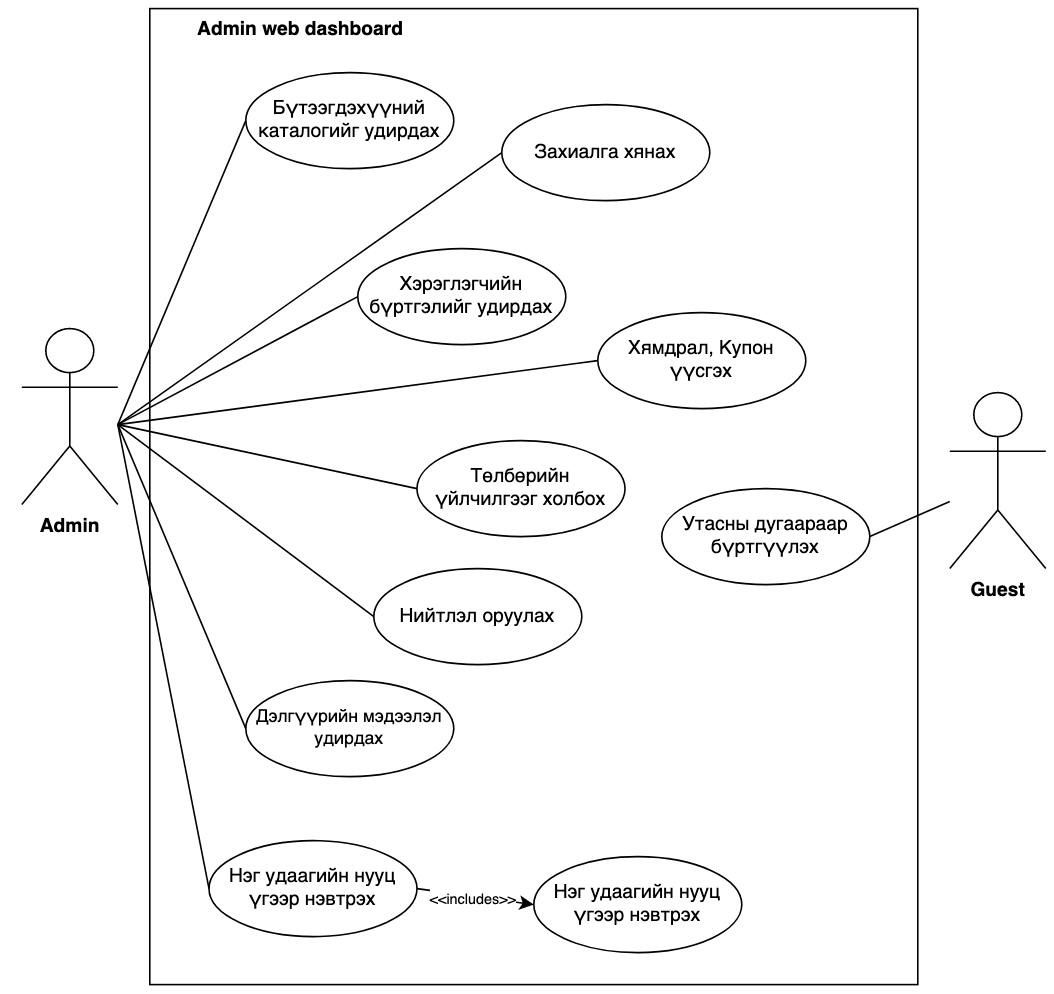
\includegraphics[scale=0.3]{src/images/usecase.png}
	\caption{Use-case диаграм}
\end{figure}
